\section{Background}
\begin{figure}
\centering
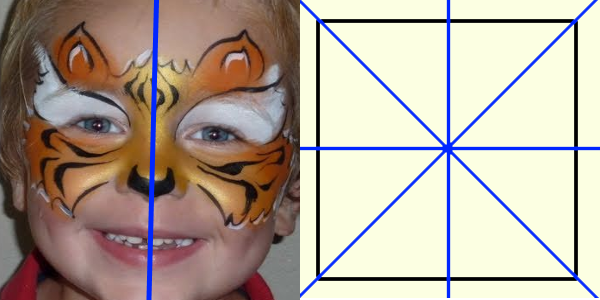
\includegraphics[width=0.9\columnwidth]{reflection}
\caption{On the left, a face, exhibiting bilateral vertical reflection symmetry. On the right, a square, which contains four reflection axes. Reflection axes are marked with blue lines. Notice that mirroring the images about any of the axes would result in the same image}
\label{ref}
\end{figure}

In two-dimensional images, there are only four transformations that are not a simple composition of other transformations. These are \textit{reflection}, \textit{rotation}, \textit{glide reflection}, and \textit{translation}. Various collections of these symmetries are what differentiate the seventeen wallpaper groups. We note that human perception does not necessarily rely on perfect symmetry. While textures which have been manipulated can pose a serious problem for computer vision algorithms, humans are quite good at recognizing patterns even in significantly distorted images \cite{nearregular}.  

Reflection is the most well-known symmetry, with the vernacular for symmetry referring exclusively to it. It refers to situations when a line can be drawn on then image, and then every point on one side of the line has a corresponding point on the other side. The clearest examples of reflection symmetry in nature are probably the faces or bodies of animals. Reflection is often referred to by the number of reflection \textit{axes}, or lines, that the object contains. A face, for instance, would only contain one. A square, on the other hand, would contain three (see Figure~\ref{ref}).

Rotation is another very common example of symmetry in nature. Rotation refers to an object's ability to rotate around some center without changing. Rotation symmetry is generally referred to by the number of rotation angles that maintain this symmetry. For instance, a hexagon has 6-fold rotation symmetry, while a flower with six pedals would have 6-fold rotation symmetry (see Figure~\ref{rot})

\begin{figure}
\centering
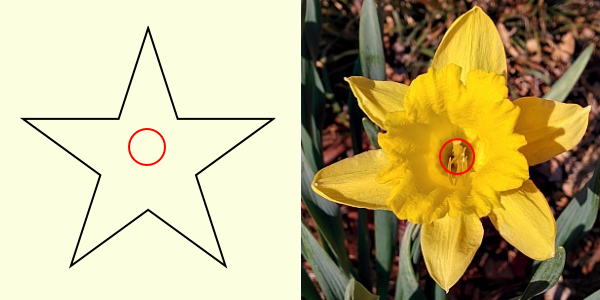
\includegraphics[width=0.9\columnwidth]{rotation}
\caption{On the left, a flower exhibiting 6-fold rotation symmetry. On the right, a five-pointed star, exhibiting 5-fold rotation symmetry. Rotation centers are marked with a red circle}
\label{rot}
\end{figure}

Translation symmetry refers to an object that repeats. For instance, in a brick wall, there are hundreds of bricks aligned in such a way that if you shifted the wall over by the length of exactly one brick, the wall would stay the same. Importantly, for this to make much sense in a mathematical sense, the wall would have to be infinitely long. Another example of translation symmetry would be a fence. If the fence was shifted by the length from one post to the next, the fence would stay the same. An important feature of translation symmetry is the \textit{tile}. The tile refers to the identical feature that is repeating. In the brick wall example, this is an individual brick, while in the fence post example, this is an individual fence post (see Figure~\ref{trans}).

\begin{figure}
\centering
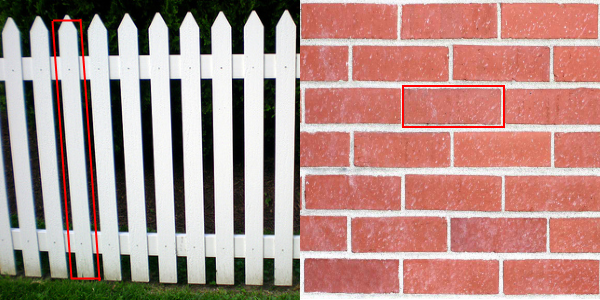
\includegraphics[width=0.9\columnwidth]{translation}
\caption{On the left, a brick wall. On the right, a white fence. In both of these images, the image would have to repeat to truly exhibit translation symmetry. The tile is outlined in red.}
\label{trans}
\end{figure}

The last basic symmetry is glide reflection. While reflection refers to something with a corresponding point directly across from it on the reflection axis, glide reflection refers to something that is reflected and then translated. The clearest examples of glide reflection in nature are footsteps. Each foot could be analyzed in terms of translation symmetry. However, halfway in between each footstep (the tile, in this case), there is a reflected footstep (made by the other foot). Thus, glide reflection is characterized by a "zig-zag" pattern of sorts, where the tile moves and reflects. Importantly, it is impossible to have glide reflection and reflection along the same axis. For instance, if someone walked some path and left footsteps that formed glide reflection, and then someone else walked along filling in a footstep that is a reflection of the original footstep, what would be left is just normal reflection, that happens twice as often as the glide reflection did (see Figure~\ref{glide}).

\begin{figure}
\centering
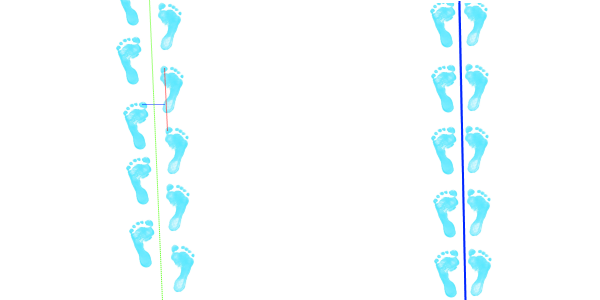
\includegraphics[width=0.9\columnwidth]{glide}
\caption{On the left, footsteps exhibiting a glide reflection pattern. On the right, footsteps exhibiting a normal reflection pattern. Note that the two by definition cannot exist along the same axis.}
\label{glide}
\end{figure}

\begin{figure}[!ht]
\centering
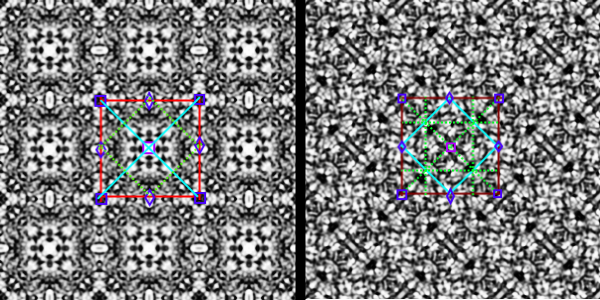
\includegraphics[width=0.9\columnwidth]{ann_images}
\caption{On the left is P4M, on the right is P4G. In each, one tile is marked with its symmetries. Notice that P4M has reflection axes on its tile border, whereas P4G does not.}
\label{fig:P4GvP4M}
\end{figure}

In the wallpaper groups, every group has translation symmetry and then a unique set of other symmetries. The seventeen groups comprise all possible sets. Table~\ref{sym-tab} gives a basic description of the seventeen groups as a set of their symmetries. Notably, sometimes even when both groups have reflection, they have it along different axes. see Figure~\ref{fig:P4GvP4M} for an example. Importantly, any single group would have the exact same symmetries, even if their appearance was different. See Figure~\ref{P4MvP4M} for an example. Every group also has its own \textit{tile shape}, which is the shape that repeats.

\begin{figure}[!ht]
\centering
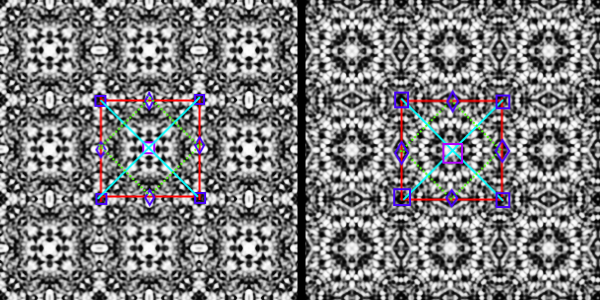
\includegraphics[width=0.9\columnwidth]{ann_images_same}
\caption{Both images are of the P4M group. Even though their appearance is quite different, they have the same symmetries in every single tile. }
\label{P4MvP4M}
\end{figure}

\begin{table}[!ht]
\centering
\resizebox{\columnwidth}{!}{%
\begin{tabular}{|l|c|c|c|c|c|c|c|c|c|}
\hline
Group & 2-fold & 3-fold & 4-fold & 6-fold & $T_1$ & $T_2$ & $D_1$ & $D_2$ &  tile \\ \hline
P1 & F & F & F & F & None & None & None & None & O \\ \hline
P2 & T & F & F & F & None & None & None & None & O \\ \hline
PM & F & F & F & F & Refl & None & None & None & Re \\ \hline
PG & F & F & F & F & Glide & None & None & None & Re \\ \hline
CM & F & F & F & F & None & None & Refl & None & Rh \\ \hline
PMM & T & F & F & F & Glide & Refl & None & None & Re \\ \hline
PMG & T & F & F & F & Glide & Refl & None & None & Re \\ \hline
PGG & T & F & F & F & Glide & Glide & None & None & Re \\ \hline
CMM & T & F & F & F & None & None & Refl & Refl & Rh \\ \hline
P4 & T & F & T & F & None & None& None & None & S \\ \hline
P4M & T & F & T & F & Refl & Refl & Refl & Refl & S \\ \hline
P4G & T & F & T & F & Glide & Glide & Refl & Refl & S \\ \hline
P3 & F & T & F & F & None & None & None & None & H \\ \hline
P3M1 & F & T & F & F & None & None & Refl& None & H \\ \hline
P31M & F & T & F & F & Refl & Refl & Refl & None & H \\ \hline
P6 & T & T & F & T & Refl & None & None & None & H \\ \hline
P6M & T & T & F & T & Refl & Refl & Refl & Refl & H \\ \hline
\end{tabular}%
}
\caption{Wallpaper groups represented as their symmetries. (Refl=Reflection, Glide=Glide Reflection, Re=Rectangular, Rh=Rhombic, O=Oblique, S=Square, H=Hexagonal)}
\label{sym-tab}
\end{table}

In representing wallpaper groups as a set of symmetries, we can then posit them in relation to each other. In this way, every group's symmetries are either a subset or a superset of every other group.  If each group is placed with its relation to other groups, they form a graph, see Figure~\ref{graph}. If an arrow points from box $A$ toward box $B$, that means that $B$'s symmetries are subset of $A$'s symmetries.


\begin{figure}[!ht]
\centering
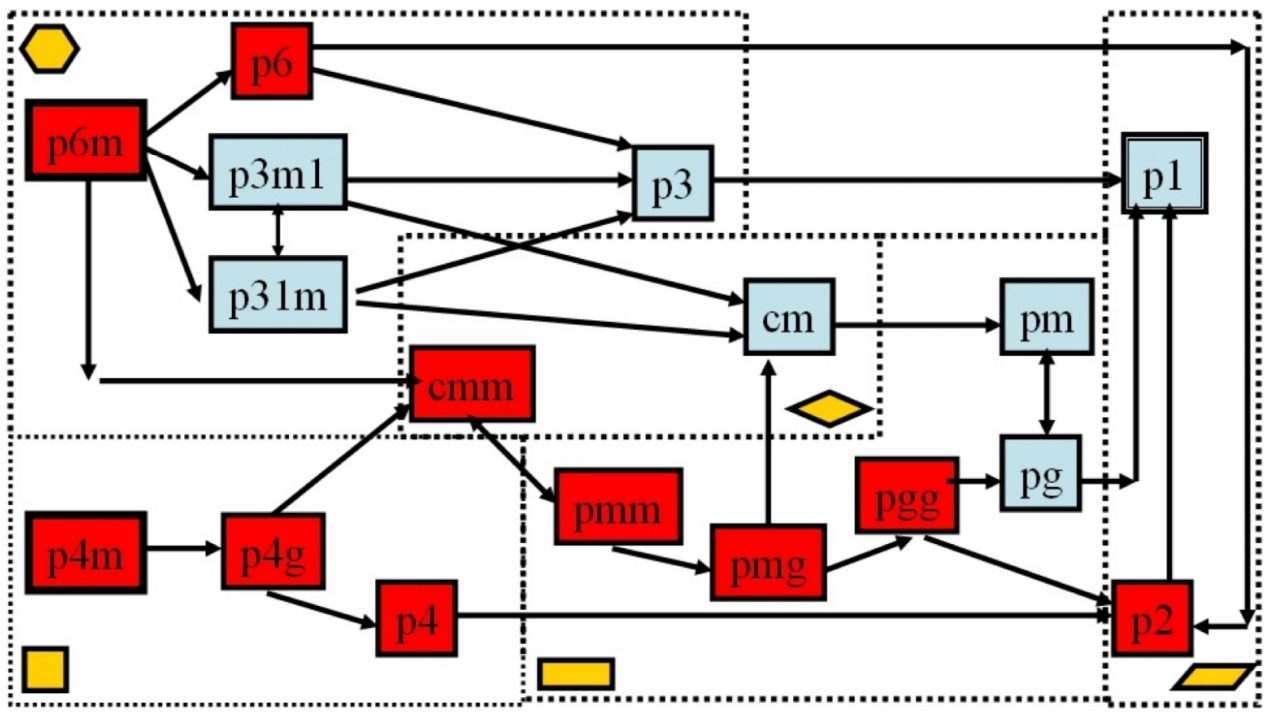
\includegraphics[width=0.9\columnwidth]{Yanxi_Graph}
\label{graph}
\caption{The subgroup relation graph}
\end{figure}